
%----------------LINEARNI-REGRESE--------------------------
\chapter{Lineární regrese}
\label{sec:LinearniRegrese}

\par{K cemu slouzi regrese}










%------------------MOTIVACE--------------------------------
\section{Motivace}
\label{sec:LinearniRegreseMotivace}

\par{Jako motivaci můžeme použít příklad, kdy si budete chtít zakoupit byt v~Plzni, proto by bylo dobré znát, kolik zaplatíte za jakou podlahovou plochu, v ideálním případě pro všechny velikosti bytů. Nebo-li se snažíte predikovat cenu bytu v~závislosti na podlahové ploše. Na Obr. \ref{fig:cena_plocha} lze vidět vývoj ceny bytu v~závislosti na podlahové ploše.}

\begin{figure}[!ht]
	\centering
	%trim option's parameter order: left bottom right top
	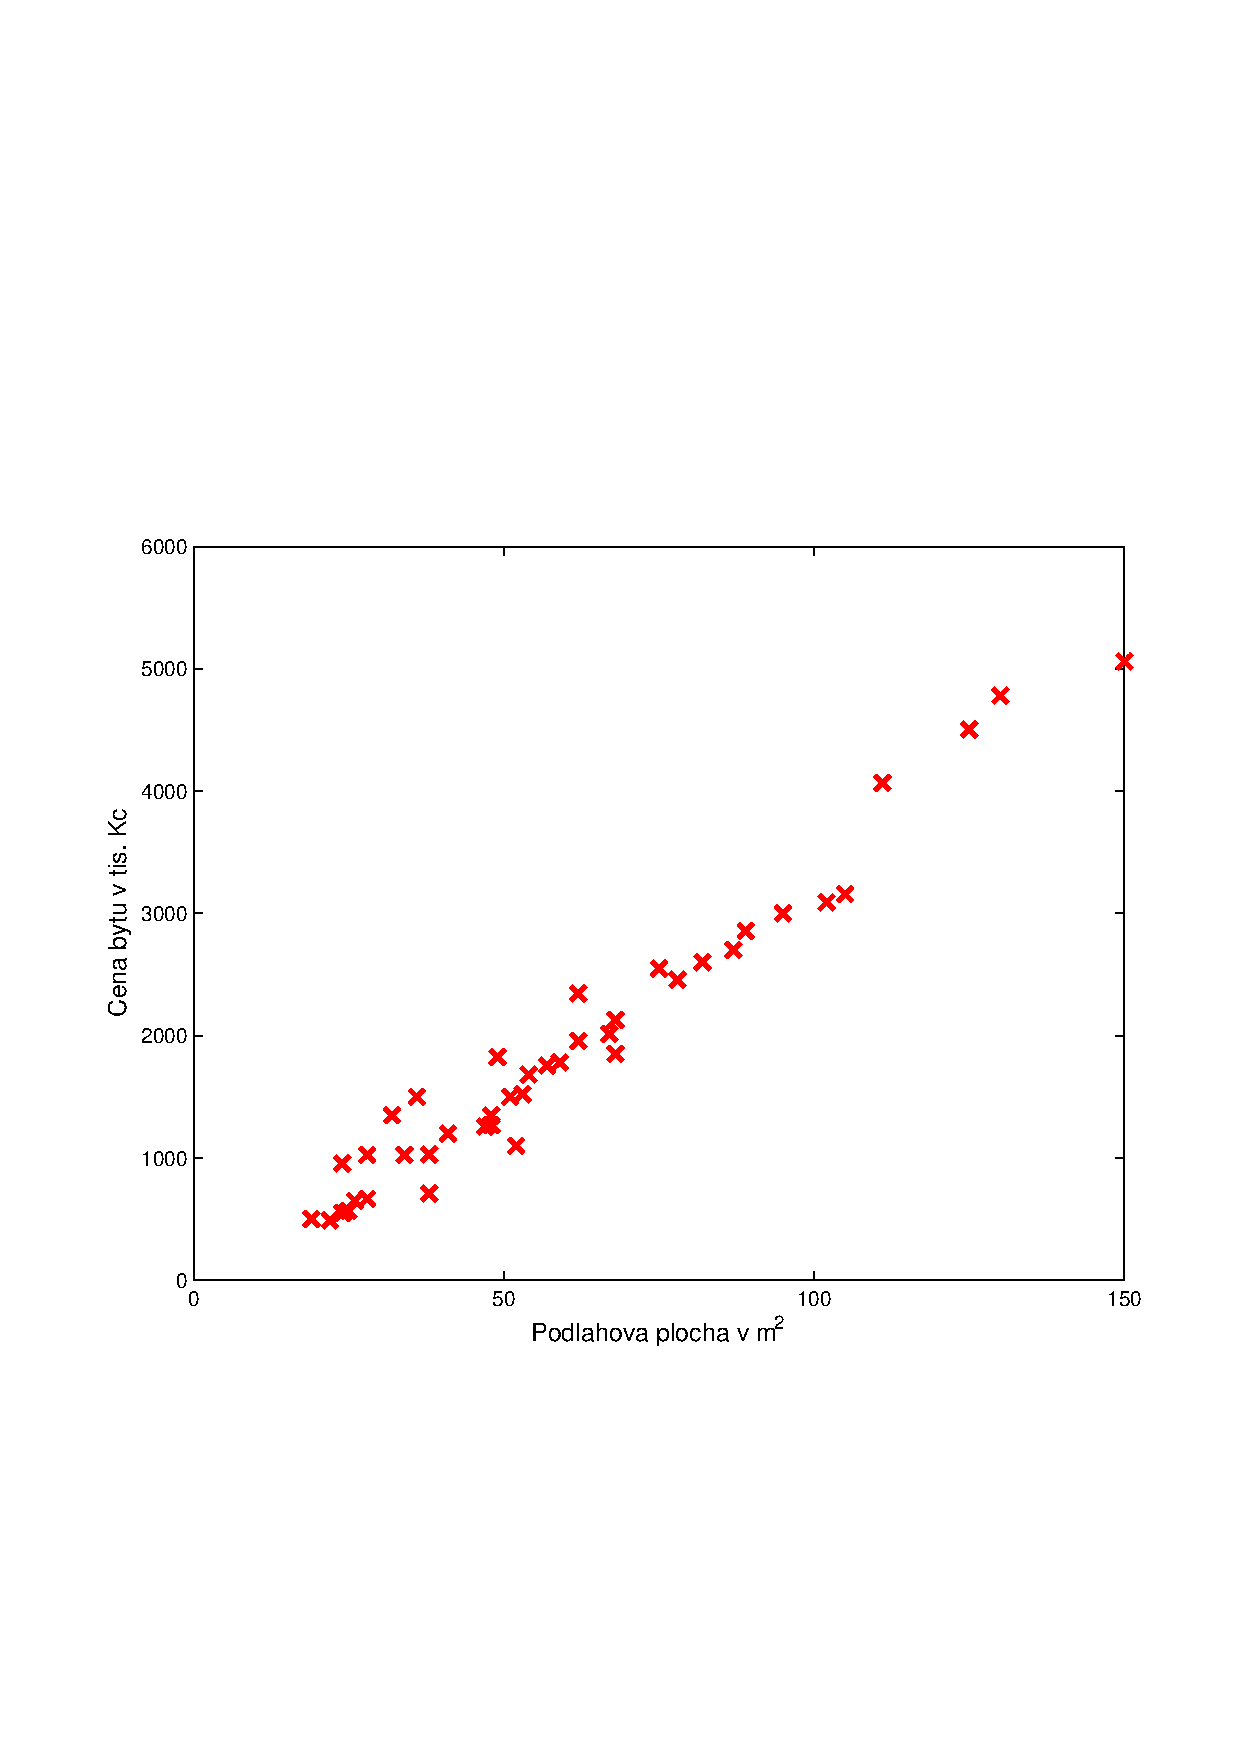
\includegraphics[scale = 0.5, trim = 3cm 7cm 3cm 9cm]{./Img/LinearniRegrese/cena_plocha.pdf}
	\caption{Vývoj ceny bytu v závislosti na podlahové ploše.}
	\label{fig:cena_plocha}
\end{figure}


\newpage




%----------------UCENI-S-UCITELEM--------------------
\section{Učení s učitelem}
\label{sec:LinearniRegreseUceniSUcitelem}

\par{Učení s~učitelem (supervised learning) dává \uv{správnou odpověď} pro každý příklad z~množiny dat.}

\par{Problém regrese: Na základě reálného (spojitého) vstupu predikovat reálný (spojitý) výstup.}

\par{Problém klasifikace: Na základě diskrétního vstupu predikovat diskrétní výstup.}

\par{Více formálně v~případě učení s~učitelem potřebujeme množinu dat nazývanou trénovací množina. V~našem případě predikce ceny bytu máme trénovací množinu cen bytů a~k~nim odpovídající podlahovou plochu. Naším úkolem je naučit se z~těchto dat jak predikovat ceny bytů.}

\par{Nyní zavedeme notaci nechť $m$ je velikost trénovací sady, $x$ jsou \uv{vstupní} proměnné neboli příznaky a~$y$ jsou \uv{výstupní} proměnné neboli příznaky. Jeden trénovací vzorek budeme označovat jako $\left(\bm{x}, y \right)$ a~odpovídá jednomu řádku v~tabulce \ref{tab:vzorky}. Dále $\left( x^{\left( i \right)}, y^{\left( i \right)} \right)$ označuje $i$-tý trénovací vzorek.}

\begin{table}[!ht]
\centering
\begin{tabular}{c|c}
	{Velikost bytu v $m^2$ ($x$)} & {Cena bytu v tis. Kč ($y$)}\\
	\hline
	{19} & {500}\\
	{22} & {490}\\
	{25} & {568}\\
	{$\ldots$} & {$\ldots$}
\end{tabular}
\caption{Příklady trénovacích vzorků.}
\label{tab:vzorky}
\end{table}

\par{Trénovací množina, v~našem případě ceny bytů, je potřebná pro natrénování učícího se algoritmu, jehož výstupem je funkce (hypotézy), která se většinou označuje $h$. Účelem funkce (hypotézy) $h$ je ze vstupu $x$ (velikost bytu) odhadnout výstup $y$ (cena bytu). Tedy $h$ je funkce, která mapuje $x$ na $y$. Schéma je naznačeno na Obr. \ref{fig:schema}.}

\begin{figure}[!ht]
	\centering
	%trim option's parameter order: left bottom right top
	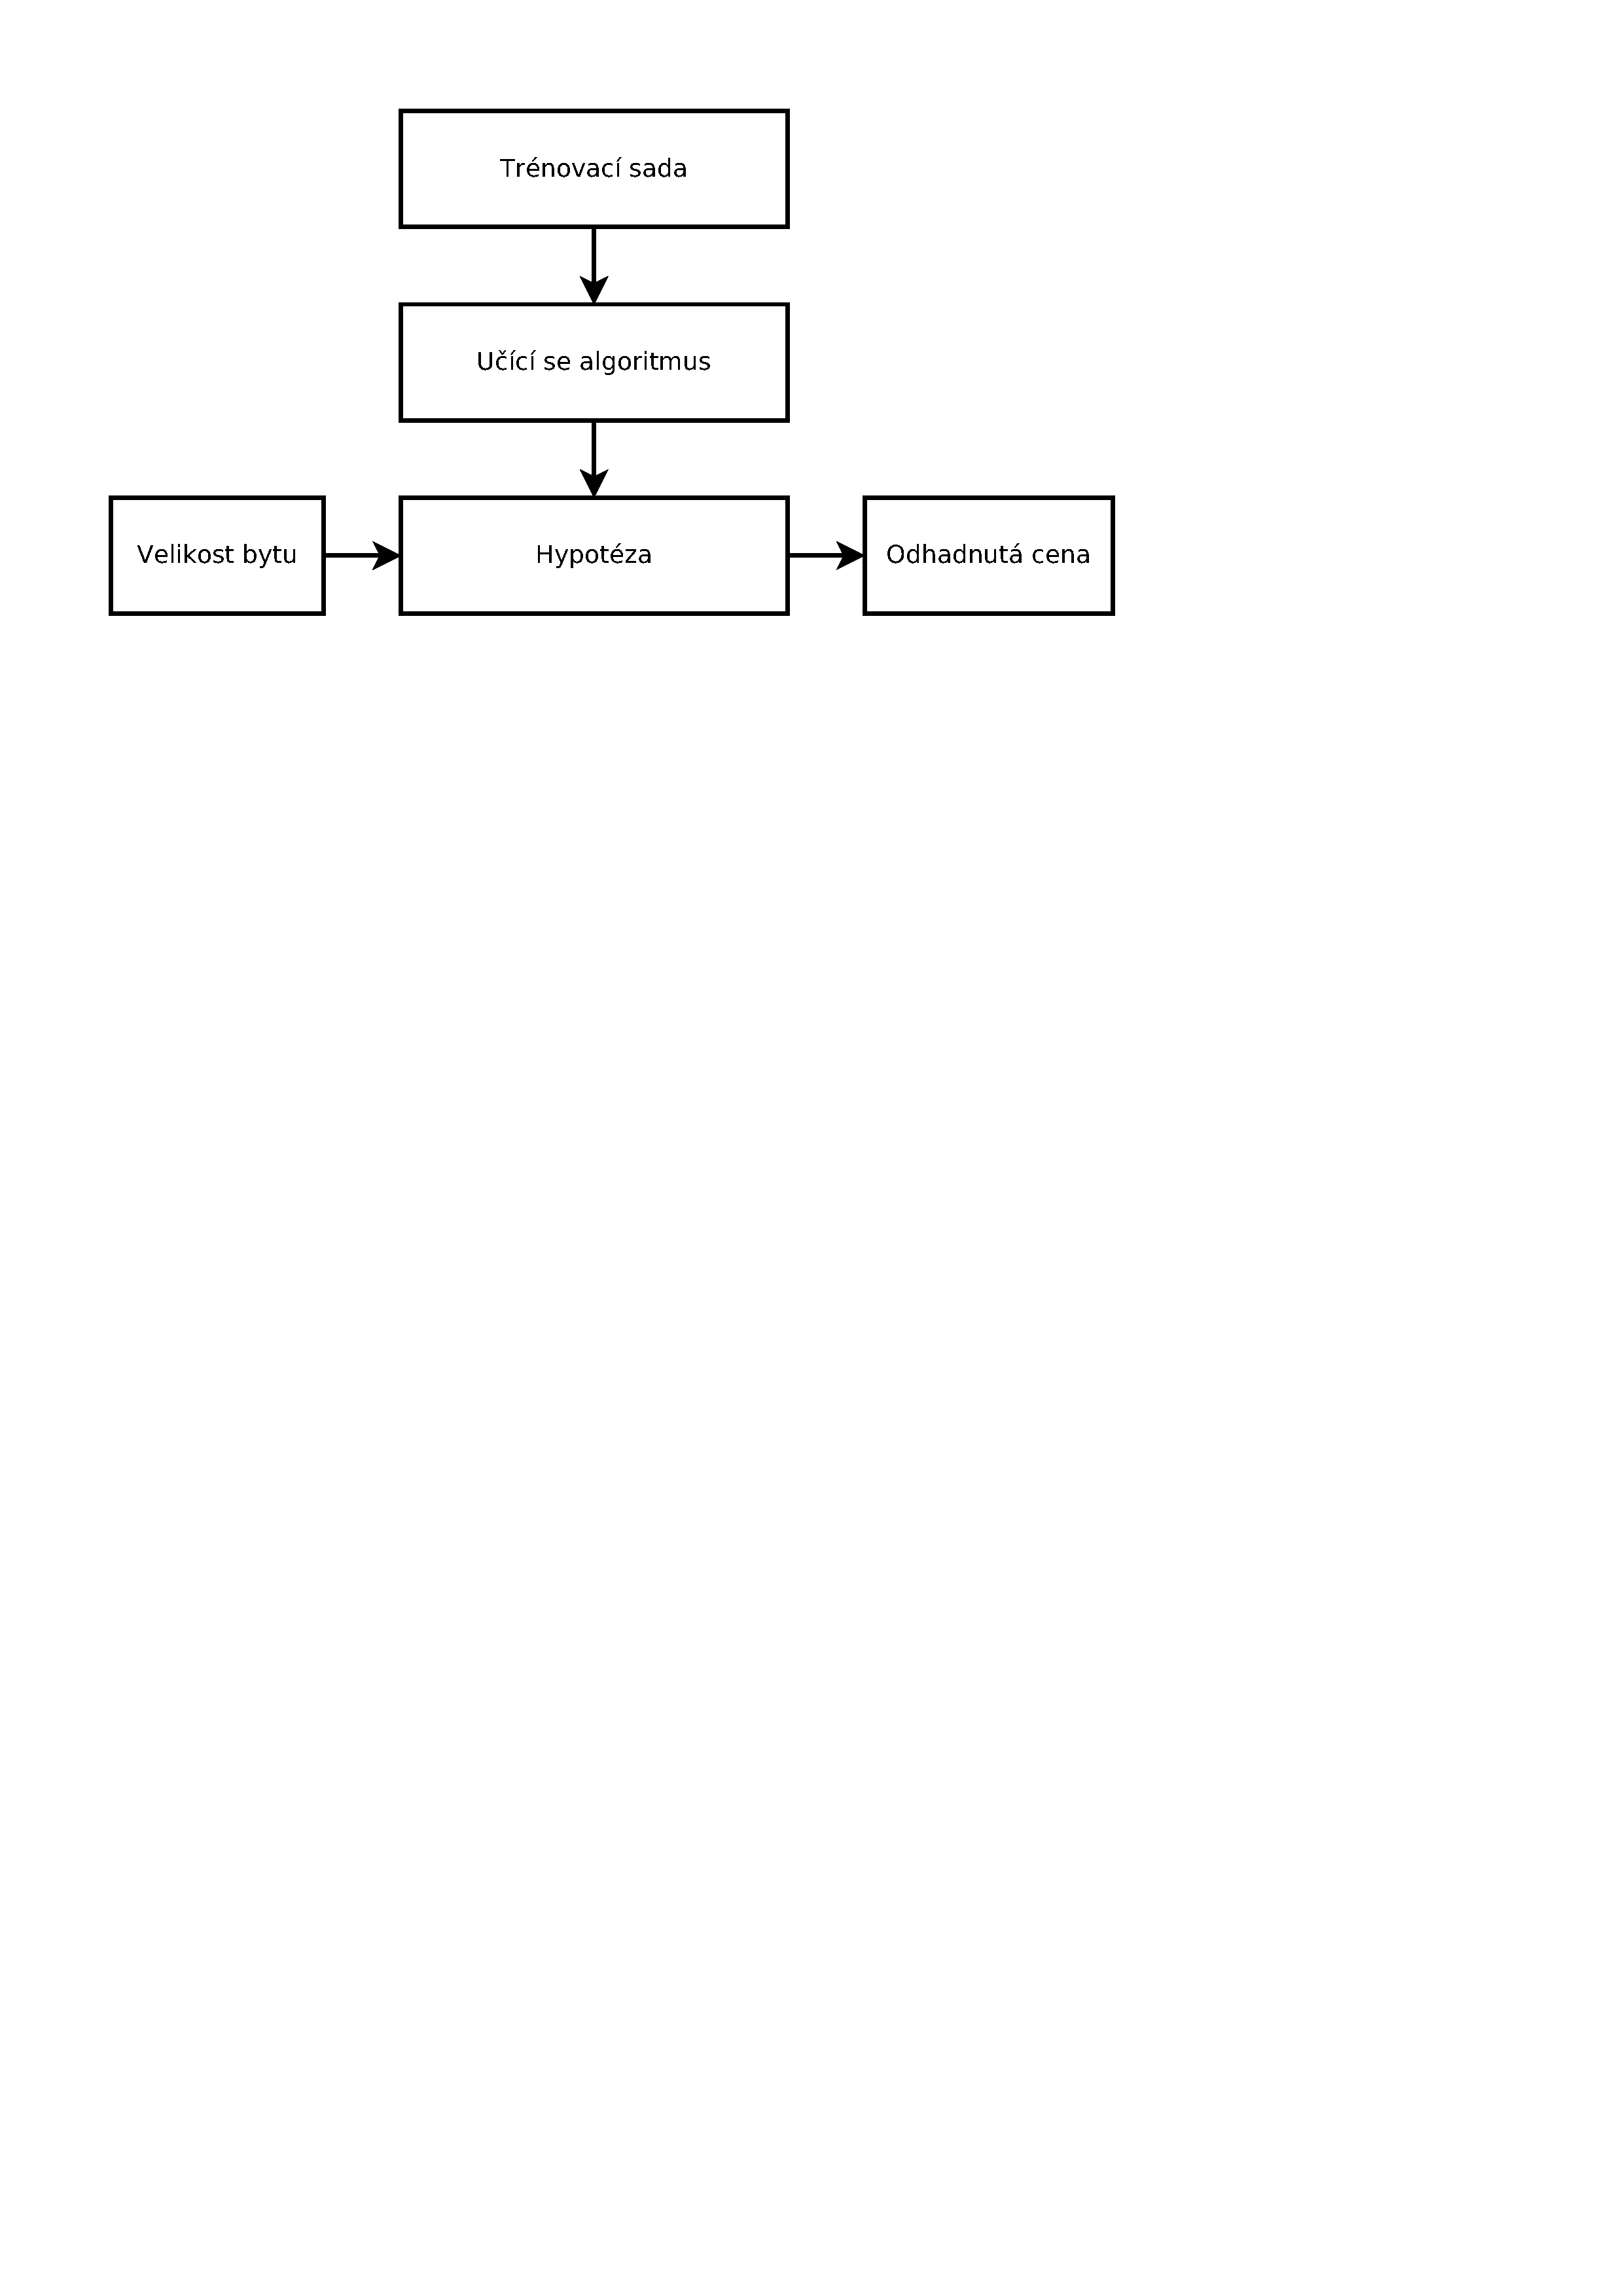
\includegraphics[scale = 0.5, trim = 3.5cm 42cm 14cm 2cm]{./Img/LinearniRegrese/schema.pdf}
	\caption{Schéma učení s učitelem.}
	\label{fig:schema}
\end{figure}

\par{Když navrhujeme učící se algoritmy, další věc kterou potřebujeme rozhodnout je jak budeme reprezentovat hypotézu $h$. V~našem motivačním příkladě si vystačíme s~hypotézou v~následujícím tvaru lineární funkce:
\begin{equation}
	h_{\bm{\Theta}} \left( x \right) = \vartheta_0 + \vartheta_1 x,
\end{equation}
zkráceně $h \left( x \right)$. Jedná se tedy o~lineární regresi s~jednou proměnnou. V~případě komplexnějšího učícího se algoritmu je nutné použít složitější nelineární model.}

\subsubsection*{Poznámka}
\par{$\vartheta$ je malá théta a $\Theta$ je velká théta.}

\newpage















%----------------ZTRATOVA-FUNKCE---------------------
\section{Ztrátová funkce}
\label{sec:LinearniRegreseZtratovaFunkce}

\par{Pro nejlepší napasování našeho lineárního modelu na trénovací data budeme potřebovat určit parametr $\vartheta_0$ a~$\vartheta_1$ v~naší hypotéze:
\begin{equation}
	h_{\bm{\Theta}} \left( x \right) = \vartheta_0 + \vartheta_1 x,
\end{equation}}

\par{Snažíme se zvolit parametry $\vartheta_0$ a $\vartheta_1$ tak, aby hypotéza $h_{\bm{\Theta}} \left( x \right)$ byla co nejblíže k $y$ pro naše trénovací vzorky $\left( x, y \right)$. Jinými slovy snažíme se minimalizovat kvadratickou chybu:

\begin{equation}
	\min_{\vartheta_0, \vartheta_1} \frac{1}{2m} \sum_{i = 1}^{m} \left( h_{\bm{\Theta}} \left( x^{\left( i \right)} \right) - y^{\left( i \right)} \right)^2,
\end{equation}
kde
\begin{equation}
	h_{\bm{\Theta}} \left( x^{\left( i \right)} \right) = \vartheta_0 + \vartheta_1 x^{\left( i \right)}.
	\label{eq:hProJednoDato}
\end{equation}
Přesněji označíme ztrátovou funkci:
\begin{equation}
	J \left( \vartheta_0, \vartheta_1 \right) = \frac{1}{2m} \sum_{i = 1}^{m} \left( h_{\bm{\Theta}} \left( x^{\left( i \right)} \right) - y^{\left( i \right)} \right)^2
\end{equation}
a minimalizujeme
\begin{equation}
	\min_{\vartheta_0, \vartheta_1} 	J \left( \vartheta_0, \vartheta_1 \right).
\end{equation}
Tato ztrátová funkce $J$ je také občas nazývána kvadratická chyba nebo ztrátová funkce kvadratické chyby.}

\par{Ztrátová funkce ve formě kvadratické chyby je nejčastěji používanou ztrátovou funkcí při řešení regresních problémů.}

\newpage









%----------------GRADIENT-DESCENT---------------------
\section{Gradientní algoritmus}
\label{sec:LinearniRegreseGradientDescent}

\par{V~kapitole \ref{sec:LinearniRegreseZtratovaFunkce} jsme definovali ztrátovou funkci $J$. V~této kapitole bude popsán gradientní algoritmus pro minimalizaci ztrátové funkce $J$. Gradientní algoritmus není omezen jen a~pouze na lineární regresi nalézá uplatnění v~optimalizaci a~v~dalších oblastech strojového učení.} 

\par{Máme ztrátovou funkci $J \left( \vartheta_0, \vartheta_1 \right)$ a~chtěli bychom jí minimalizovat. Proto zvolíme náhodně $\vartheta_0$ a~$\vartheta_1$, dále v~každé iteraci měníme hodnoty $\vartheta_0$ a~$\vartheta_1$, tak abychom redukovali $J \left( \vartheta_0, \vartheta_1 \right)$ dokud, v~nejlepším případě, nedokonvergujeme do globálního minima.}

\par{Obecně lze gradientní algoritmus použít na jakoukoliv ztrátovou funkci:
\begin{equation}
	J \left( \vartheta_0, \cdots, \vartheta_n \right)
\end{equation}
a snažíme se minimalizovat:
\begin{equation}
	\min_{\vartheta_0, \ldots, \vartheta_n} J \left( \vartheta_0, \ldots, \vartheta_n \right)
\end{equation}}

\par{Definice gradientního algoritmu: opakuj dokud není dosaženo konvergence
\begin{equation}
	\vartheta_j = \vartheta_j - \alpha \frac{\partial}{\partial \vartheta_j} J \left( \vartheta_0 , \vartheta_1 \right),
	\label{eq:gradDescentIter}
\end{equation}
pro $j = \{ 0, 1 \}$, pro náš příklad (lineární regrese jedné proměnné) v~sekci \ref{sec:LinearniRegreseMotivace}. V~rovnici \ref{eq:gradDescentIter} proměnná $\alpha$ určuje, jak velké kroky bude gradientní algoritmus dělat při hledání minima a~nazývá se rychlost učení. V~případě velké hodnoty $\alpha$ bude algoritmus postupovat velkými kroky, rychle, ale není zajištěna konvergence, jelikož se může stát, že algoritmus bude kroužit kolem minima, ale nedosáhne ho, nebo bude divergovat. V~případě malé hodnoty $\alpha$ bude algoritmus velice pomalý a~nemusí dosáhnout minima pro stanovený počet iterací. Gradientní algoritmus může konvergovat do lokálního minima v~případě, že je rychlost učení $\alpha$ konstantní. Proto se v~reálných aplikacích volí nejdříve větší $\alpha$, které se s~rostoucí hodnotou iterací nebo času zmenšuje.}

\subsubsection*{Poznámka}
\par{Pro implementaci: je nutné aktualizovat všechny $\Theta$ současně
\begin{eqnarray}
	&temp_0 &= \vartheta_0 - \alpha \frac{\partial}{\partial \vartheta_0} J \left( \vartheta_0 , \vartheta_1 \right),\\
	&temp_1 &= \vartheta_1 - \alpha \frac{\partial}{\partial \vartheta_1} J \left( \vartheta_0 , \vartheta_1 \right), \\
		&\vartheta_0 &= temp_0, \\
		&\vartheta_1 &= temp_1.
\end{eqnarray}}

\par{Nyní budeme aplikovat gradientní algoritmus na náš problém lineární regrese
\begin{equation}
	\frac{\partial}{\partial \vartheta_j} J \left( \vartheta_0, \vartheta_1 \right) = \frac{\partial}{\partial \vartheta_j} \cdot \frac{1}{2m} \sum_{i = 1}^{m} \left( h_{\bm{\Theta}} \left( x^{\left( i \right)} \right) - y^{\left( i \right)} \right)^2,
\end{equation}
po dosazení z~rovnice \ref{eq:hProJednoDato} dostáváme
\begin{equation}
	\frac{\partial}{\partial \vartheta_j} J \left( \vartheta_0, \vartheta_1 \right) = \frac{\partial}{\partial \vartheta_j} \cdot \frac{1}{2m} \sum_{i = 1}^{m} \left( \vartheta_0 + \vartheta_1  x^{\left( i \right)} - y^{\left( i \right)} \right)^2,
\end{equation}
po zderivování podle jednotlivých parametrů $\Theta$ získáme
\begin{eqnarray}
	\frac{\partial}{\partial \vartheta_0} &J \left( \vartheta_0, \vartheta_1 \right) &= \frac{1}{m} \sum_{i = 1}^{m} \left( h_{\bm{\Theta}} \left( x^{\left( i \right)} \right) - y^{\left( i \right)} \right),\\
	\frac{\partial}{\partial \vartheta_1} &J \left( \vartheta_0, \vartheta_1 \right) &= \frac{1}{m} \sum_{i = 1}^{m} \left( h_{\bm{\Theta}} \left( x^{\left( i \right)} \right) - y^{\left( i \right)} \right) x^{\left( i \right)}.
\end{eqnarray}}

\par{Výsledný konkrétní tvar rovnice \ref{eq:gradDescentIter} pro $\vartheta_0$ a $\vartheta_1$
\begin{eqnarray}
		&\vartheta_0 &= \vartheta_0 - \alpha \frac{1}{m} \sum_{i = 1}^{m} \left( h_{\bm{\Theta}} \left( x^{\left( i \right)} \right) - y^{\left( i \right)} \right),\\
		&\vartheta_1 &= \vartheta_1 - \alpha \frac{1}{m} \sum_{i = 1}^{m} \left( h_{\bm{\Theta}} \left( x^{\left( i \right)} \right) - y^{\left( i \right)} \right) x^{\left( i \right)}.
\end{eqnarray}}

\par{Gradientnímu algoritmu popsanému výše se také někdy říká dávkový gradientní algoritmus, protože využívá všechna trénovací data, při součtu přes všech $m$ vzorků, v~každém kroku.}

\begin{figure}[!ht]
	\centering
	%trim option's parameter order: left bottom right top
	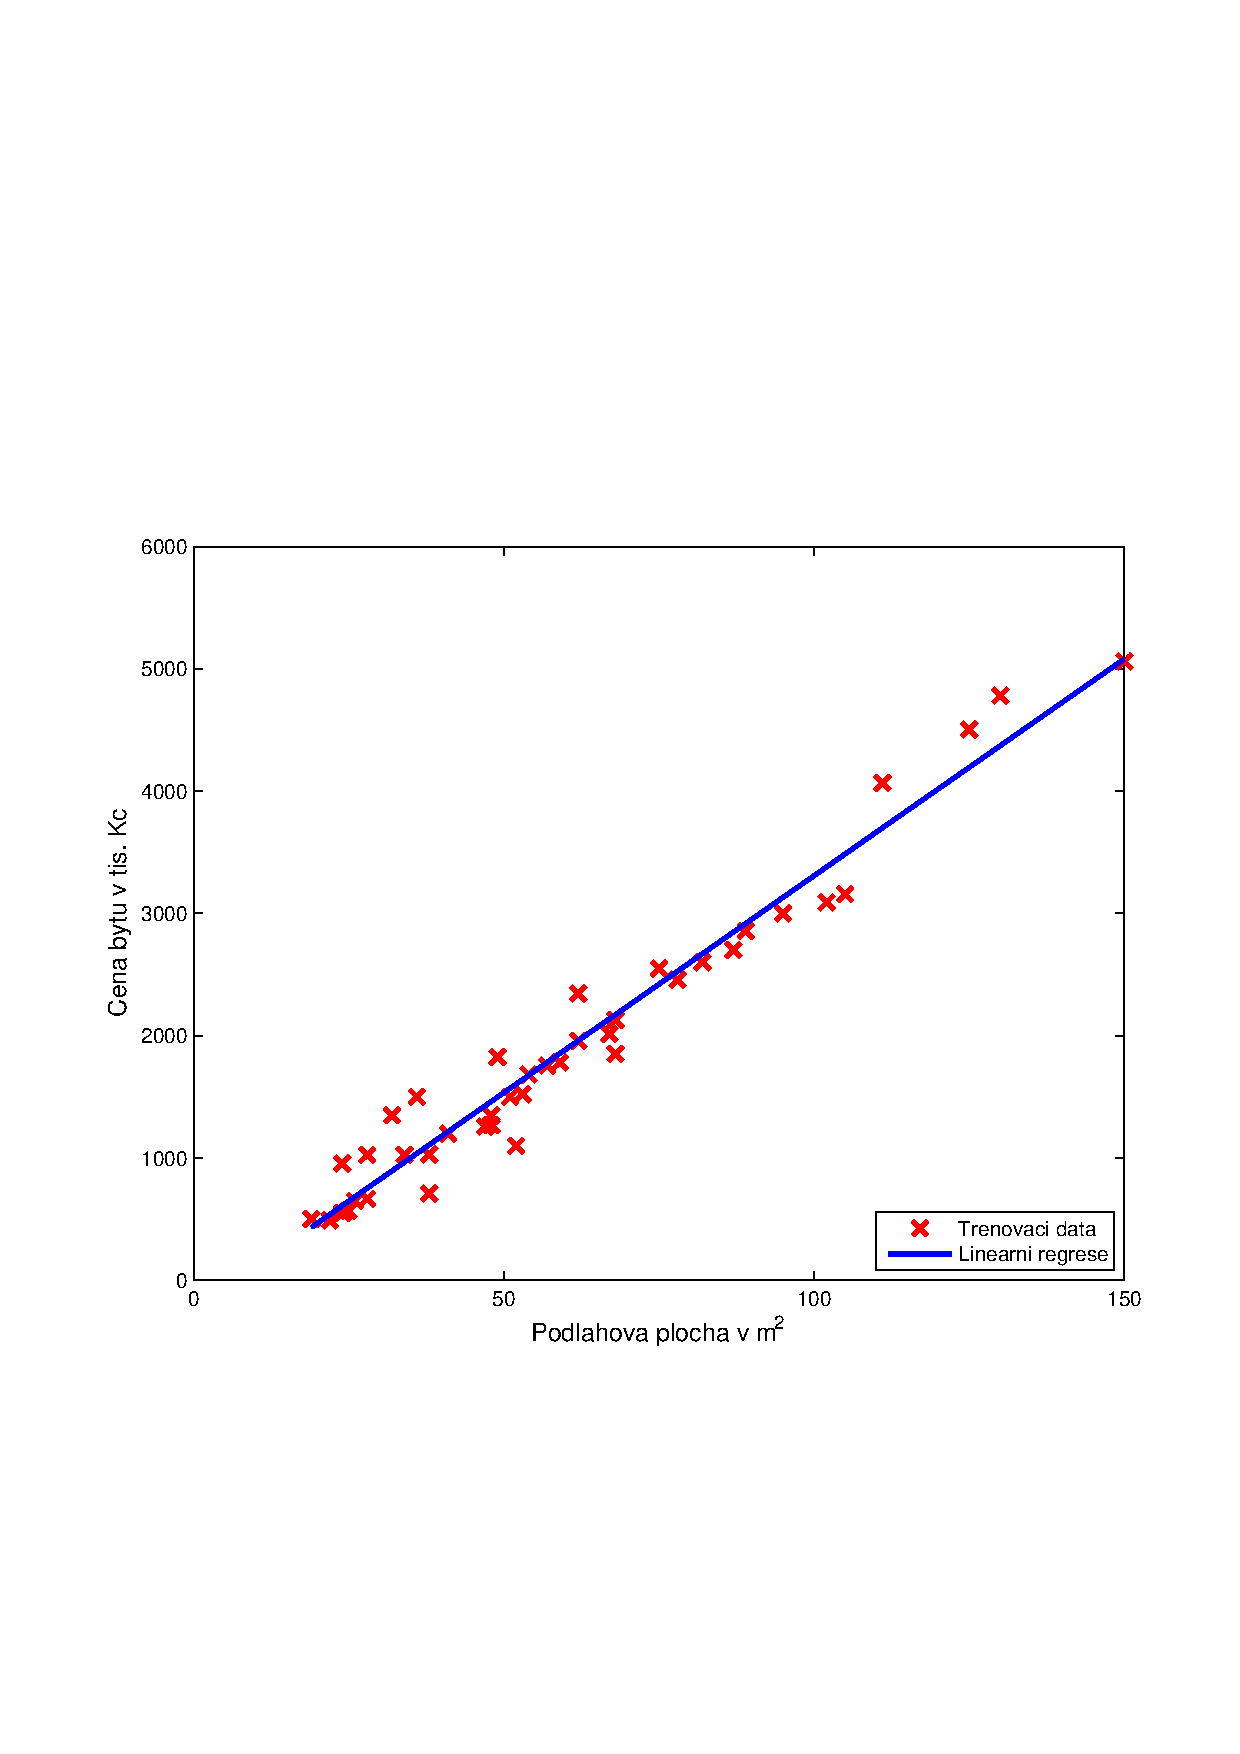
\includegraphics[scale = 0.5, trim = 2.5cm 7cm 2cm 9cm]{./Img/LinearniRegrese/cena_plocha_linear_regrese.pdf}
	\caption{Výsledná lineární regrese našeho úvodního příkladu po výpočtu gradientním algoritmem.}
	\label{fig:cena_plocha_linear_regrese}
\end{figure}


\newpage









%----------------VICEROZMERNA-LINEARNI-REGRESE-------------------
\section{Vícerozměrná lineární regrese}
\label{sec:LinearniRegreseVicePromennych}

\par{V sekci \ref{sec:LinearniRegreseUceniSUcitelem} byla představena lineární regrese o~jedné proměnné na příkladě predikce ceny bytu (výstup $y$) v závislosti na velikosti podlahové plochy $m^2$ (vstup $x$).}

\par{V případě vícerozměrné lineární regrese si můžeme představit, že nemáme pouze velikost podlahové plochy bytu, ale výsledná cena závisí i dalších parametrech bytu, viz tabulka \ref{tab:vzorkyND}.

\begin{table}[!ht]
\centering
\begin{tabular}{c|c|c|c|c}
	{Velikost bytu} & {Počet místností} & {Počet poschodí} & {Stáří bytu} & {Cena bytu}\\
	{$x_1$} & {$x_2$} & {$x_3$} & {$x_4$} & {$y$}\\
	\hline
	{19} & {5} & {1} & {45} & {500}\\
	{22} & {3} & {2} & {40} & {490}\\
	{25} & {2} & {1} & {30} & {568}\\
	{$\ldots$} & {$\ldots$} & {$\ldots$} & {$\ldots$} & {$\ldots$}
\end{tabular}
\caption{Příklady vícerozměrných trénovacích vzorků.}
\label{tab:vzorkyND}
\end{table}}

\par{Proměnnou $n$ budeme označovat počet příznaků (v~našem případě v tabulce \ref{tab:vzorkyND} $x_{1, \ldots , 4}$, proto $n = 4$.) Dále budeme stále jako u jednorozměrného případu označovat vstupní příznaky (všechny = sloupcový vektor) $\bm{x}^{\left( i \right)}$ pro $i$-tý trénovací vzor. A~hodnota jednotlivého $j$-tého příznaku $i$-tého trénovacího vzoru bude označována $\bm{x}^{\left( i \right)}_{j}$.}

\par{V~případě jednorozměrné lineární regrese byla naše hypotéza $h_\Theta$ reprezentována
\begin{equation}
	h_{\bm{\Theta}} \left( x \right) = \vartheta_0 + \vartheta_1 x,
	\label{eq:1Dhypothesis}
\end{equation}
v~našem vícerozměrném případě nabývá tvaru
\begin{equation}
	h_{\bm{\Theta}} \left( \bm{x} \right) = \vartheta_0 + \vartheta_1 x_1 + \vartheta_2 x_2 + \vartheta_3 x_3 + \vartheta_4 x_4 .
	\label{eq:NDhypothesis}
\end{equation}
V~případě \ref{eq:1Dhypothesis} i \ref{eq:NDhypothesis} je možné si všimnout, že $x_0 = 1$ čehož dále využijeme, přesněji $\bm{x}^{\left( i \right)}_0 = 1$ z důvodu dodržení konvence. Proto $\bm{x} \in \mathrm{R}^{n + 1}$ a to samé platí pro parametry $\bm{\Theta} \in \mathrm{R}^{n + 1}$.}

\subsubsection*{Poznámka}
\par{V~našem příkladě odpovídají
\begin{equation}
	\bm{x} = \left[ x_0,~x_1,~x_2,~x_3,~x_4 \right]^{\top}
\end{equation}
a
\begin{equation}
	\bm{\Theta} = \left[ \vartheta_0,~\vartheta_1,~\vartheta_2,~\vartheta_3,~\vartheta_4 \right]^{\top}.
\end{equation}}

\par{Obecněji lze vícerozměrnou hypotézu zapsat jako
\begin{equation}
	h_{\bm{\Theta}} \left( \bm{x} \right) = \vartheta_0 + \vartheta_1 x_1 + \vartheta_2 x_2 + \ldots + \vartheta_n x_n,
	\label{eq:NDhypothesisObecne}
\end{equation}
neboli jednoduše jako součin vektorů (vnitřní produkt)
\begin{equation}
	h_{\bm{\Theta}} \left( \bm{x} \right) = \bm{\Theta}^{\top} \bm{x}.
	\label{eq:NDhypothesisObecneVektorove}
\end{equation}}


\newpage












%----------------GRADIENT-DESCENT-VICEROZMERNY--------------------
\section{Gradientní algoritmus - vícerozměrná verze}
\label{sec:LinearniRegreseGradientDescentVicerozmerny}

\par{Budeme potřebovat hypotézu
\begin{equation}
	h_{\bm{\Theta}} \left( \bm{x} \right) = \bm{\Theta}^{\top} \bm{x} = \vartheta_0 x_0 + \vartheta_1 x_1 + \vartheta_2 x_2 + \ldots + \vartheta_n x_n,
\end{equation}
kde $x_0 = 1$, dále parametry $\bm{\Theta} = \left[ \vartheta_0,~\vartheta_1,~\vartheta_2,~\ldots,~\vartheta_4 \right]^{\top}$ a vícerozměrnou ztrátovou funkci
\begin{equation}
	J \left( \bm{\Theta} \right) = \frac{1}{2m} \sum_{i = 1}^{m} \left( h_{\bm{\Theta}} \left( \bm{x}^{\left( i \right)} \right) - y^{\left( i \right)} \right)^2.
\end{equation}}

\par{Gradientní algoritmus pak bude mít tvar: opakuj
\begin{equation}
	\vartheta_j = \vartheta_j - \alpha \frac{\partial}{\partial \vartheta_j} J \left( \bm{\Theta} \right),
	\label{eq:algoritmusNDgradientDescent}
\end{equation}
současně aktualizovat parametry pro všechny $j = 0, \ldots, n$.}

\par{Vztah z rovnice \ref{eq:algoritmusNDgradientDescent} lze zapsat jako
\begin{equation}
	\frac{\partial}{\partial \vartheta_j} J \left( \bm{\Theta} \right) = \frac{1}{m} \sum_{i = 1}^{m} \left( h_{\bm{\Theta}} \left( \bm{x}^{\left( i \right)} \right) - y^{\left( i \right)} \right) \bm{x}^{\left( i \right)}_j
	\label{eq:derivaceNDgradientDescent}	
\end{equation}
a po spojení rovnic 	\ref{eq:algoritmusNDgradientDescent} a \ref{eq:derivaceNDgradientDescent} získáváme výsledný tvar
\begin{equation}
	\vartheta_j = \vartheta_j - \alpha \frac{1}{m} \sum_{i = 1}^{m} \left( h_{\bm{\Theta}} \left( \bm{x}^{\left( i \right)} \right) - y^{\left( i \right)} \right) \bm{x}^{\left( i \right)}_j,
	\label{eq:NDgradientDescentVysledna}
\end{equation}
pokud bychom výslednou rovnici \ref{eq:NDgradientDescentVysledna} rozepsali pro první dva parametry $\vartheta_0$ a $\vartheta_1$ dostali bychom
\begin{eqnarray}
	&\vartheta_0 &= \vartheta_0 - \alpha \frac{1}{m} \sum_{i = 1}^{m} \left( h_{\bm{\Theta}} \left( \bm{x}^{\left( i \right)} \right) - y^{\left( i \right)} \right) \bm{x}^{\left( i \right)}_0, \quad \bm{x}^{\left( i \right)}_0 = 1\\
	&\vartheta_1 &= \vartheta_1 - \alpha \frac{1}{m} \sum_{i = 1}^{m} \left( h_{\bm{\Theta}} \left( \bm{x}^{\left( i \right)} \right) - y^{\left( i \right)} \right) \bm{x}^{\left( i \right)}_1\\
	\nonumber
	&\vdots
\end{eqnarray}}


\newpage













%----------------FEATURES-SCALING-------------------
\section{Features scaling}
\label{sec:featuresScaling}

\par{V~této podkapitole si řekneme něco o~velikosti příznaků. První a~nejdůležitější věcí je normování velikostí příznaků na stejnou velikost. Neboli, pokud použijeme opět náš příklad nákupu bytu a~definujeme si velikost bytu v~$dm^2$ (příznak $x_1$) a~počet místností bytu (příznak $x_2$) a~řekněme že:
\begin{eqnarray}
	\nonumber
	&x_1 &\in \langle 5000, 20000 \rangle,\\
	\nonumber
	&x_2 &\in \langle 1, 5 \rangle,
\end{eqnarray}
tak bude pro gradientní metodu velmi obtížné a~více výpočetně náročné (bude nutno spočítat více iterací) nalézt minimum. Proto je důležité, aby všechny příznaky měli stejné škálování. V~našem případě by to znamenalo 

\begin{eqnarray}
	\nonumber
	&x_1 &= \frac{\mbox{velikost bytu}}{20000},\\
	\nonumber
	&x_2 &= \frac{\mbox{počet místností}}{5}.
\end{eqnarray}
Více obecně lze říci, že se většinou volí normování na interval $\langle -1, 1 \rangle$.}

\subsubsection*{Mean normalization}
\par{Velice častá normalizace střední hodnotou $\mu$, konkrétně pro $i$-tý příznak
\begin{equation}
	x_i \leftarrow \frac{x_i - \mu_i}{max - min}
\end{equation}
nebo
\begin{equation}
	x_i \leftarrow \frac{x_i - \mu_i}{std}
\end{equation}
($std$ = Standard deviation).


\newpage















%----------------NORMAL-EQUATION------------------
\section{Analytické řešení}
\label{sec:normalEquation}

\par{V této sekci si ukážeme jak lze vypočítat minimum naší ztrátové funkce $J \left( \bm{\Theta} \right)$ analyticky.}

\subsubsection*{Příklad:}
\par{Předpokládejme 1D příklad ($\vartheta \in \mathcal{R}$), kdy máme ztrátovou funkci $J \left( \vartheta \right)$, která je funkcí jedné reálné proměnné
\begin{equation}
	J \left( \vartheta \right) = a \vartheta^2 + b \vartheta + c
\end{equation}}

\par{Pro minimalizaci naší kvadratické ztrátové funkce využijeme hledání extrému (položíme derivaci rovnou nule)
\begin{equation}
	\frac{\mathrm{d}}{\mathrm{d}\vartheta} J \left( \vartheta \right) = \ldots \equiv 0
\end{equation}
a vyřešíme pro parametr $\vartheta$.}

\par{Více obecněji pro $\bm{\Theta} \in \mathcal{R}^{n+1}$ bude naše ztrátová funkce nabývat tvaru
\begin{equation}
	J \left( \vartheta_0,~\vartheta_1,~\ldots,~\vartheta_m \right) = \frac{1}{2m} \sum_{i=1}^{m} \left( h_{\bm{\Theta}} \left( \bm{x}^{\left( i \right)} \right) - y^{\left( i \right)} \right)^2
\end{equation}
dále položíme parciální derivace podle jednotlivých parametrů rovny nule (pro všechny $j$)
\begin{equation}
	\frac{\partial}{\partial \vartheta_j} = \ldots \equiv 0
\end{equation}
a vyřešíme pro parametry $\vartheta_0,~\vartheta_1,~\ldots,~\vartheta_m$.}

\par{Pro složení obyčejné rovnice budeme potřebovat matici $\bm{X} \in \mathcal{R}^{m \times \left( n + 1 \right)}$, která v řádcích obsahuje jednotlivé vektory $\left( \bm{x}^{\left( i \right)} \right)^{\top}$ a výstupní sloupcový vektor $\bm{y} \in \mathcal{R}^{m}$. Kde $m$ je počet trénovacích vzorků (velikost trénovací množiny) a $n$ je počet příznaků, kde $\bm{x}_0^{\left( i \right)} = 0$.}

\par{Nyní můžeme zapsat předpis pro výpočet parametrů $\bm{\Theta}$ analyticky
\begin{equation}
	\bm{\Theta} = \left( \bm{X}^{\top} \bm{X} \right)^{-1} \bm{X}^{\top} \bm{y}.
\end{equation}
Pro analytické řešení není nutné příznaky normovat, jako v případě gradientního algoritmu, na stejné měřítko, jak je popsáno v sekci \ref{sec:featuresScaling}.}

\newpage




















%----------------NORMAL-EQUATION------------------
\section{Gradientní algoritmus vs. analytické řešení}
\label{sec:GAvsAR}

\par{V této sekci budou zmíněny výhody a nevýhody gradientního algoritmu versus analytického řešení. Velikost trénovací množiny $m$ a počet příznaků $n$.
\begin{center}
\begin{tabular}{c|c}
	{Gradientní algoritmus} & {Analytické řešení} \\
	\hline
	{Nutno zvolit konstantu učení $\alpha$.} & {Není nutné volit konstantu učení $\alpha$.}\\
	{Potřebuje mnoho iterací.} & {Nepotřebuje iterovat.}\\
	{Pracuje dobře, když je $n$ velké.} & {Pomalé pokud je $n$ velké.}\\
	{~} & {Nutnost vypočítat inverzi $\left( \bm{X}^{\top} \bm{X} \right)^{-1}$.}\\
	{~} & {(Složitost $\mathcal{O}\left( n^3 \right)$).}\\
	{Zvolit pokud $n > 10^6$.} & {Zvolit pokud $n < 10^4$.}
\end{tabular}
\end{center}}


\newpage













